\documentclass[110pt, oneside]{article}   	% use "amsart" instead of "article" for AMSLaTeX format
\usepackage[margin=0.75in]{geometry}            		% See geometry.pdf to learn the layout options. There are lots.
\geometry{letterpaper}                   		% ... or a4paper or a5paper or ... 
%\geometry{landscape}                		% Activate for rotated page geometry
%\usepackage[parfill]{parskip}    		% Activate to begin paragraphs with an empty line rather than an indent
\usepackage{graphicx}				% Use pdf, png, jpg, or eps§ with pdflatex; use eps in DVI mode
								% TeX will automatically convert eps --> pdf in pdflatex		
\usepackage{amssymb}
\usepackage{float}

%SetFonts

%SetFonts


\title{Logistic Regression Analysis, CSCI 5622 Homework 2 \vspace{-2ex} }
\author{Alex Gendreau \vspace{-2ex}}
\date{\vspace{-2ex}}							% Activate to display a given date or no date

\begin{document}
\maketitle \vspace{-2ex}
%\section{}
%\subsection{}


\begin{enumerate}
\item \textbf {What is the role of the learning rate?} \\
\begin{figure}[H]
\centering
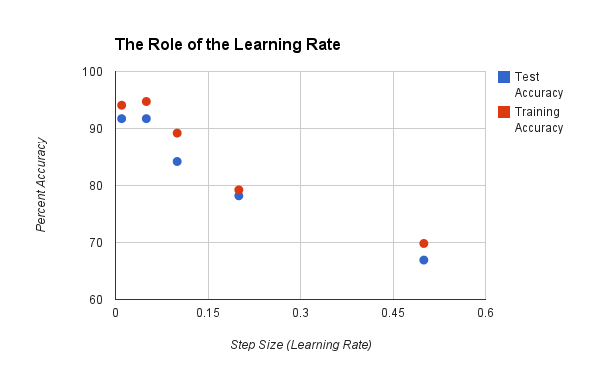
\includegraphics[scale=0.3]{learningRate.png}
\caption{The percent accuracy of both the training and test sets based on varying the step size (the learning rate) for regularized logistic regression, $\mu=0.01$.}
\end{figure}

\item \textbf{How many passes over the data do you need to complete?}\\
\begin{figure}[H]
\centering
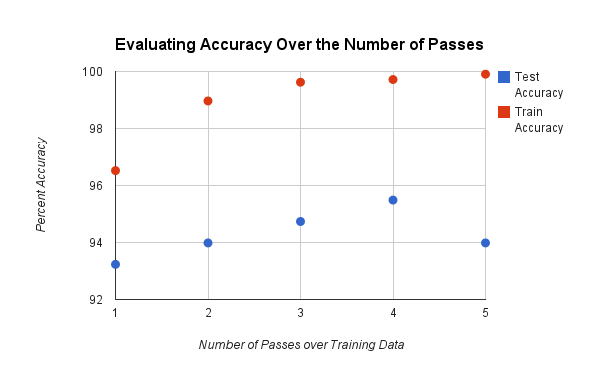
\includegraphics[scale=0.3]{passes.png}
\caption{The percent accuracy of both the training and test sets based on varying the number of passes over the training set.}
\end{figure}

We conducted an experiment using the default settings (i.e. $\mu=0$ and a learning rate of $0.1$) while varying the number of passes and examining the accuracy of both the training set and the test set.  In Figure $1$, we see that the while the training set increase in accuracy for all passes (as expected since we are running multiple passes on the training set), the accuracy of the test set increases until the fourth pass but actually decrease on the fifth pass.  One reason for this is that we are overfitting the training set with five passes.  From the experiment, I would suggest 4 passes over the training set on the default settings for generating the best logistic function.

\item \textbf{What words are the best predictor of each class?}\\
Using the default settings, I found the best predictors for \textbf{baseball were: pitching, saves, bat, runs, and hit}.  The best predictors for \textbf{hockey were: hockey, playoffs, pick, playoff, and points}.  To find these values I looked at the features that had the largest coefficients (betas) for baseball and the smallest coefficients (betas) for hockey.  I chose to use this as my metric for best features because features with large coefficients (either positive or negative) give greater weight to the logistic function.  I accessed these words using the argsort function in python which returns a list of the indices of the of an array in sorted order.  These indices correspond to feature numbers, which then allowed me to access the features.
\item \textbf{What words are the poorest predictors of classes?}\\
Using the default settings, I found the worst predictors were: \textbf{racist, bloody, blasted, hooked, and intermissions}.  To find these values I looked the feature coefficients with the smallest absolute value.  These features would contribute least the logistic function and thus the classification process.  I used a similar implementation to access the smallest in absolute value coefficients by first taking the absolute value of all the feature coefficients (betas).  
\end{enumerate}









\end{document}  